\documentclass{standalone}

\usepackage{tikz}
\usepackage{xcolor}
\definecolor{primary}{HTML}{003262} % berkeley blue
\definecolor{secondary}{HTML}{FDB515} % cal gold
\definecolor{founder}{HTML}{3B7EA1}
\definecolor{medalist}{HTML}{C4820E}
\definecolor{goldengate}{HTML}{ED4E33}
\definecolor{ion}{HTML}{CFDD45}

\begin{document}
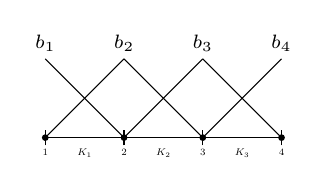
\begin{tikzpicture}
	\def\gap{.1cm}
	\scriptsize
	\draw (0,-.1) grid (3,.1); 
	\foreach \i in {1,...,3}{
		\node[scale=.5] at (\i-.5,-.2) {$K_{\i}$}; 
	}
	\foreach \i in {1,...,4}{
		\filldraw (\i-1,0) circle[radius=1pt] node[below=\gap, scale=.5] {\i}; 
		\node at (\i-1,1.2) {$b_\i$}; 
	}

	\foreach \i in {0,...,2}{
		\draw (\i,0) -- (\i+1,1); 
		\draw (\i,1) -- (\i+1,0); 
	}

	% \begin{scope}[yshift=-2cm]
	% 	\draw (0,-.1) grid (3,.1); 
	% 	% \foreach \i in {1,...,6}{
	% 	% 	\node[scale=.5] at (\i-.5,-.35) {$K_{\i}$}; 
	% 	% }
	% 	\foreach[evaluate=\i as \x using (\i-1)*3/6] \i in {1,...,7}{
	% 		\filldraw (\x,0) circle[radius=1pt] node[below=\gap, scale=.5] {\i}; 
	% 		\node at (\x,1.2) {$b_\i$}; 
	% 	}

	% 	\foreach \e in {0,...,2}{
	% 		\draw[domain=0:1, smooth, xshift=\e cm] plot(\x,{(\x-1)*(\x-.5)*2}); 
	% 		\draw[domain=0:1, smooth, xshift=\e cm] plot(\x,{\x*(\x-.5)*2}); 
	% 		\draw[domain=0:1, smooth, xshift=\e cm] plot(\x,{\x*(1-\x)*4}); 
	% 	}
	% \end{scope}

	% \begin{scope}[yshift=-4cm]
	% 	\draw (0,-.1) grid (3,.1); 
	% 	\foreach \e in {0,...,2}{
	% 		\foreach \i [count=\j from 3*\e+1] in {0,.276393,.723606}{
	% 			\filldraw (\e+\i,0) circle[radius=1pt] node[below=\gap, scale=.5] {\j}; 
	% 		}
	% 	}
	% 	\filldraw (3,0) circle[radius=1pt] node[below=\gap, scale=.5] {10}; 

	% 	\foreach \e in {0,...,2}{
	% 		\draw[domain=0:1, smooth, xshift=\e cm] plot(\x, {-5*\x^3 + 10*\x^2 - 6*\x + 1});
	% 		\draw[domain=0:1, smooth, xshift=\e cm] plot(\x, {5*\x^3 - 5*\x^2 + 1*\x});
	% 		\draw[domain=0:1, smooth, xshift=\e cm] plot(\x, {11.1803399*\x^3 - 19.2705098*\x^2 + 8.09016994*\x}); 
	% 		\draw[domain=0:1, smooth, xshift=\e cm] plot(\x, {-11.1803399*\x^3 + 14.2705098*\x^2 - 3.09016994*\x}); 
	% 	}
	% \end{scope}
\end{tikzpicture}
\end{document}